\subsection{Linear Regression}

Linear Regression is a statistical technique used to model the relationship between a dependent variable (Y) and one or more independent variables (X). It helps us understand how the dependent variable changes when the independent variables change. This method is commonly used in predictive analytics and inferential statistics.

\subsection*{Key Concepts}

\begin{itemize}
    \item \textbf{R\textsuperscript{2} (R-Squared):} R² measures the proportion of variance in the dependent variable that is explained by the independent variables in the model. Think of R² as a score from 0 to 1 that tells you how well your model fits the data.
    \begin{itemize}
        \item An R² of 0.80 means your model explains 80\% of the changes in the result (e.g., temperature). 
        \item The closer to 1, the better your model is at predicting.
    \end{itemize}

    \item \textbf{p-value:} The p-value tests the null hypothesis that a coefficient is equal to zero (i.e., no effect). A value less than 0.05 typically indicates statistical importance. The p-value tells you how likely it is that the result happened by chance.
    \begin{itemize}
        \item If it’s less than 0.05, the variable likely has a real effect on the result. 
        \item For example, a p-value of 0.01 means there’s a very low chance that the result is random.
       \end{itemize}
    \item \textbf{$\boldsymbol{\beta}$ Coefficients:} Beta coefficients represent the estimated change in the dependent variable for a one-unit increase in the independent variable, holding other variables constant. This tells you how much the output will go up or down when the input changes.
    \begin{itemize}
        \item If $\beta = 0.6$ for humidity, then for every 1\% rise in humidity, the temperature increases by 0.6°C (assuming other things stay the same). \item Positive $\beta$ means increase, negative $\beta$ means decrease.
      \end{itemize}
    \item \textbf{Residual Plots:} Residual plots show the difference between observed and predicted values. Random scatter suggests a good model fit. A residual plot is like a ``reality check'' for your model.
    \begin{itemize}
        \item It shows how far off your predictions are.
        \item If the errors (dots) are randomly scattered, it means your model is doing a fair job without obvious bias or patterns.
    \end{itemize}

\end{itemize}

\subsection*{Steps to Perform Linear Regression}

\begin{enumerate}
    \item Click on the \textbf{Regression} tab in the top menu.
    \item Select \textbf{Linear Regression} from the dropdown list.
    \item Drag your dependent variable (Y) (e.g., Temperature) into the \textbf{Dependent Variable} box.
    \item Drag one or more independent variables (X) (e.g., Humidity, Pressure, Precipitation) into the \textbf{Covariates} box.
\end{enumerate}

% Figure here-----------------------------
\begin{figure}[h]
\centering
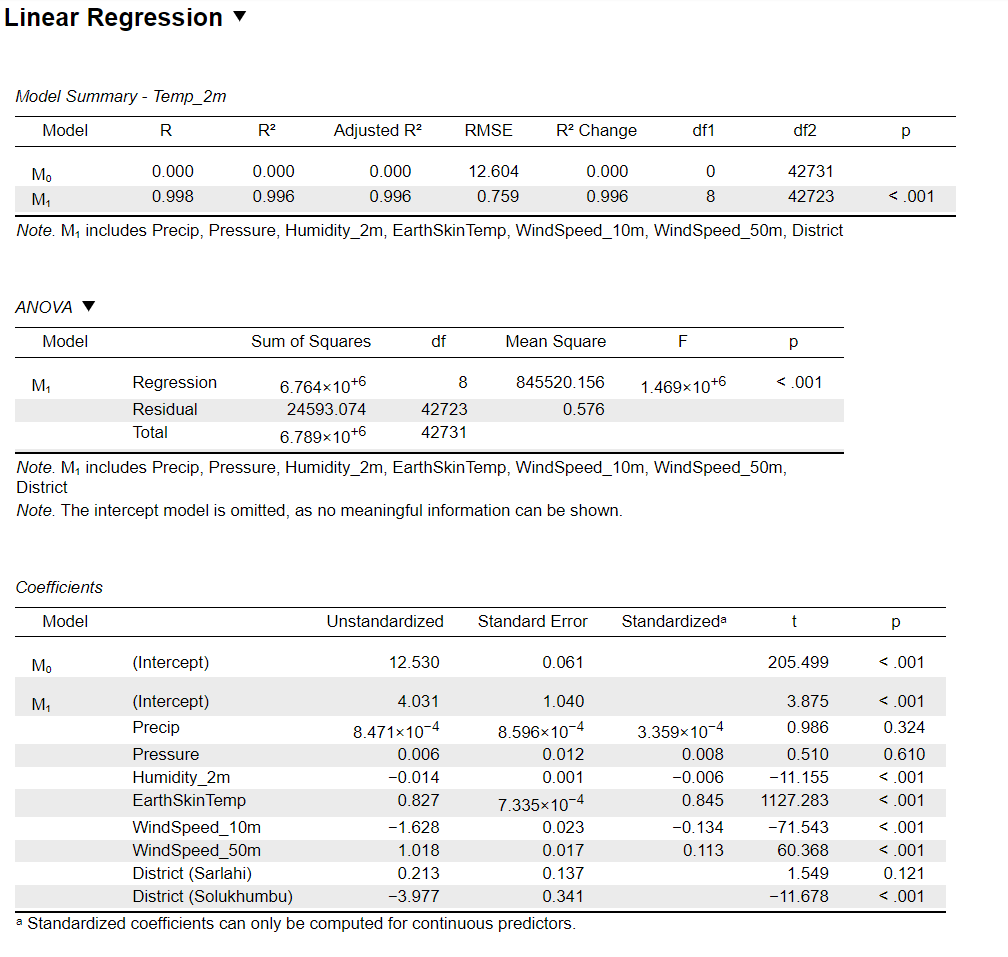
\includegraphics[width=0.7\textwidth]{figures/regression_jasp.png}
\caption{Linear Regression Model Summary}
\end{figure}

\textbf{Interpretation:}
\begin{itemize}
    \item \textbf{Model Summary}
    \begin{itemize}
        \item The model includes 8 predictors: \textit{Precipitation, Pressure, Humidity\_2m, EarthSkinTemp, WindSpeed\_10m, WindSpeed\_50m, District (Sarlahi, Solukhumbu)}.
        \item $R^2 = 0.996$ — the model explains 99.6\% of the variation in temperature.
        \item RMSE (Root Mean Square Error) = 0.759 — the average error in temperature prediction is around $0.76^\circ$C.
        \item The model is statistically significant: $p < .001$.
    \end{itemize}
    \item \textbf{ANOVA Table}
    \begin{itemize}
        \item The model overall is highly significant: $F = 1.469 \times 10^6$, $p < .001$.
        \item This indicates that the combination of predictors meaningfully explains temperature variation.
    \end{itemize}

    \item \textbf{Important Predictors}
    \begin{enumerate}
        \item \textbf{Significant predictors} ($p < .05$):
        \begin{itemize}
            \item EarthSkinTemp — strongest predictor ($t = 1127.283$, $p < .001$)
            \item WindSpeed\_10m and WindSpeed\_50m — both have significant negative effects.
            \item Humidity\_2m — significant negative effect ($p < .001$)
            \item District (Solukhumbu) — significantly colder than the reference district ($t = -11.678$, $p < .001$)
        \end{itemize}
        \item \textbf{Non-significant predictors}:
        \begin{itemize}
            \item Precipitation ($p = 0.324$)
            \item Pressure ($p = 0.610$)
            \item District (Sarlahi) — not significantly different from Kathmandu ($p = 0.121$)
        \end{itemize}
    \end{enumerate}
\end{itemize}

% Figure here-----------------------------
\begin{figure}[h]
\centering
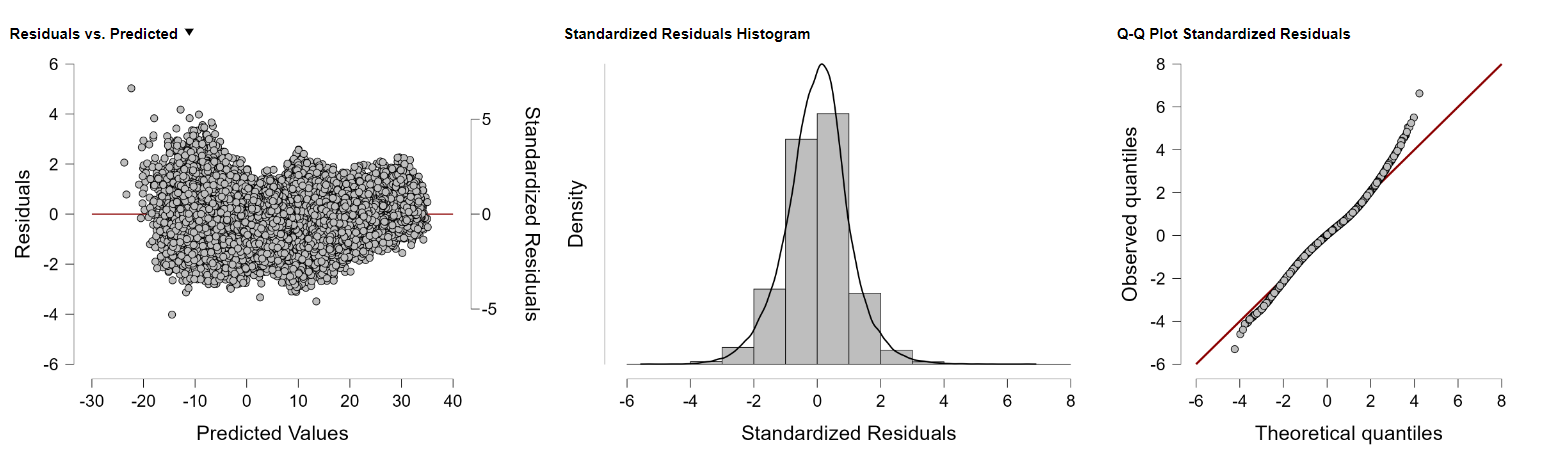
\includegraphics[width=0.7\textwidth]{figures/regression_plot.png}
\caption{Residual Plots}
\end{figure}

\textbf{Residual Diagnostics (Model Assumptions)}
    \begin{itemize}
        \item \textbf{Residuals vs. Predicted}:
        \begin{itemize}
            \item Shows a funnel-shaped spread, suggesting possible heteroscedasticity (non-constant variance).
        \end{itemize}
        \item \textbf{Histogram of Standardized Residuals}:
        \begin{itemize}
            \item Residuals are approximately normally distributed — a good sign.
        \end{itemize}
        \item \textbf{Q-Q Plot}:
        \begin{itemize}
            \item Points follow the straight line closely, indicating residuals are mostly normal, with a few outliers.
        \end{itemize}
    \end{itemize}

The regression model predicts temperature very well using weather and geographic factors. Earth Skin Temperature and Wind Speed are the most important predictors. While the model fits well and errors are mostly normal, the spread of residuals shows a bit of unevenness, which might need attention in further analysis.

